\documentclass{article}

% if you need to pass options to natbib, use, e.g.:
% \PassOptionsToPackage{numbers, compress}{natbib}
% before loading nips_2017
%
% to avoid loading the natbib package, add option nonatbib:
% \usepackage[nonatbib]{nips_2017}

\usepackage[final]{nips_2017}

% to compile a camera-ready version, add the [final] option, e.g.:
% \usepackage[final]{nips_2017}

\usepackage[utf8]{inputenc} % allow utf-8 input
\usepackage[T1]{fontenc}    % use 8-bit T1 fonts
\usepackage{hyperref}       % hyperlinks
\usepackage{url}            % simple URL typesetting
\usepackage{booktabs}       % professional-quality tables
\usepackage{amsfonts}       % blackboard math symbols
\usepackage{nicefrac}       % compact symbols for 1/2, etc.
\usepackage{microtype}      % microtypography
\usepackage{amsmath}
\usepackage{subcaption}
\usepackage{natbib}

\usepackage{graphicx}

\title{Predicting Future Machine Failure from Machine State Using Logistic Regression}

% The \author macro works with any number of authors. There are two
% commands used to separate the names and addresses of multiple
% authors: \And and \AND.
%
% Using \And between authors leaves it to LaTeX to determine where to
% break the lines. Using \AND forces a line break at that point. So,
% if LaTeX puts 3 of 4 authors names on the first line, and the last
% on the second line, try using \AND instead of \And before the third
% author name.

\author{
  Matthew Battifarano\\
  Department of Civil and Environmental Engineering\\
  Carnegie Mellon University\\
  \texttt{mbattifa@andrew.cmu.edu} \\
  %% examples of more authors
   \And
  David DeSmet \\
  Department of Civil and Environmental Engineering \\
  Carnegie Mellon University \\
  \texttt{ddesmet@andrew.cmu.edu} \\
  \And
  Achyuth Madabhushi\\
  Department of Civil and Environmental Engineering\\
  Carnegie Mellon University  \\
  \texttt{amadabhu@andrew.cmu.edu} \\
  \AND
  Parth Nabar \\
  Department of Civil and Environmental Engineering\\
  Carnegie Mellon University\\
  \texttt{pnabar@andrew.cmu.edu} \\
  %% \And
  %% Coauthor \\
  %% Affiliation \\
  %% Address \\
  %% \texttt{email} \\
}

\begin{document}
% \nipsfinalcopy is no longer used

\maketitle

\begin{abstract}
  Accurately predicting machine failures in advance can decrease maintenance cost and help allocate maintenance resources more efficiently. Logistic regression was applied to predict machine state 24 hours in the future given the current machine state.
\end{abstract}


\section{Introduction}
Understanding and predicting machine failure has become a crucial aspect of business operations. 45\% of all maintenance efforts are ineffective and 30\% of maintenance activities happen too frequently \cite{IBM-machinefailure}. A data-driven approach to predict machine failure reduces the time and cost burden associated with machine failure. Logistic Regression (LR) is a widely-used data-driven approach to binary classification. LR linearly classifies data into identifiable areas where distance from a decision boundary dictates the probability of inclusion within the class. \cite{Shalizi2012}

Prior literature has also used Support Vector Machines (SVM) to predict failures in server systems \cite{Murray2005} and hard-drives \cite{Turnbull2003}. However, SVM, unlike LR, does not provide readily interpretable outcomes that can be provided to a domain expert. 

\section{Methods}

Individual datasets were merged to construct an event stream of machine state. This event stream was used in a logistic regression model to predict the failure of the machine 24 hours in the future. The data was fit using the \texttt{LogisticRegression} model provided by the \texttt{scikit-learn} library. \cite{scikit-learn} A Jupyter notebook\cite{Kluyver2016} with the code used to generate results and figures in this report can be found on GitHub. \cite{2018HackAuton} 

\subsection{Data processing}

The data is composed of several different streams of machine events, identified by the timestamp of the observation, rounded to the hour, and an integer identifier of the machine. These datasets were merged together on observation time and machine identifier to construct an event stream of the complete machine state. Table \ref{tab:datasets} enumerates the datasets and their schemas.

\begin{table}[!ht]
\centering
\caption{Dataset schemas}
\label{tab:datasets}
\begin{tabular}{lll}
\toprule
dataset & field & description\\
\midrule
failures 	&				& event stream of component failures\\
			& machine\_id 	& unique machine identifier\\
			& datetime 		& the observation timestamp\\
            & comp\_1		& whether or not component 1 failed\\
            & comp\_2		& whether or not component 2 failed\\
            & comp\_3		& whether or not component 3 failed\\
            & comp\_4		& whether or not component 4 failed\\
\midrule
errors		&				& event stream of non-failure error codes\\
			& machine\_id 	& unique machine identifier\\
			& datetime 		& the observation timestamp\\
            & error\_1		& whether or not error 1 occurred\\
            & error\_2		& whether or not error 2 occurred\\
            & error\_3		& whether or not error 3 occurred\\
            & error\_4		& whether or not error 4 occurred\\
            & error\_5		& whether or not error 5 occurred\\
\midrule
maintenance	& 				& component maintenance records\\
			& machine\_id 	& unique machine identifier\\
			& datetime 		& the maintenance timestamp\\
            & comp\_1		& whether or not component 1 was replaced\\
            & comp\_2		& whether or not component 2 was replaced\\
            & comp\_3		& whether or not component 3 was replaced\\
            & comp\_4		& whether or not component 4 was replaced\\
            & comp\_1\_fail	& whether or not component 1 was replaced due to failure\\
            & comp\_2\_fail	& whether or not component 2 was replaced due to failure\\
            & comp\_3\_fail	& whether or not component 3 was replaced due to failure\\
            & comp\_4\_fail	& whether or not component 4 was replaced due to failure\\
\midrule
telemetry 	&				& physical measurements of the machine\\
			& machine\_id 	& unique machine identifier\\
			& datetime 		& the observation timestamp\\
            & volt			& voltage measurements\\
            & rotate		& rotation measurements\\
            & pressure		& pressure measurements\\ 
            & vibration		& vibration measurements\\
\midrule
machines	&				& description of each machine\\
			& machine\_id	& unique machine identifier\\
            & age			& age of the machine in years\\
            & model\_1		& whether or not the machine is a model 1\\
            & model\_2		& whether or not the machine is a model 2\\
            & model\_3		& whether or not the machine is a model 3\\
            & model\_4		& whether or not the machine is a model 4\\
\bottomrule
\end{tabular}
\end{table}

The event stream of the complete machine state is constructed by joining the telemetry, maintenance, and errors datasets together on machine\_id and datetime. Since telemetry contains measurements every hour for one year, event records are left joined to telemetry. The left join ensures that non-events (e.g. times at which no events occurred) are included in the event stream. The machines dataset is joined in to add age and model type to the data. Finally the day of week is extracted from the timestamp of each data point and included as a categorical feature.

Machine failure is defined as the event that at least one of its four components has failed as reported in the failures dataset. The target variable is defined as the machine failure state 24 hours after the measurement timestamp of each data point in the event steam. 

\subsection{Logistic regression}

Logistic regression is a commonly used classification method known for its easily interpretable model parameters. \cite{Agresti2003}\cite{Shalizi2012} Logistic regression models the probability of a binary target variable $Y$ given the features $X$ by mapping a linear combination of the features to $(0, 1)$ via a non-linear transformation function given by \eqref{eqn:logisitic-regression-model}.

\begin{align}
	P(Y=1 \mid X=x) = \pi(x) &= \frac{\exp(\alpha + \beta^Tx)}{1+\exp(\alpha + \beta^Tx)} \label{eqn:logisitic-regression-model}
\end{align}

In this context, each $x$ is a vector containing the complete machine state of a single machine at a single point in time and the target variable, $y$, represents the failure state of the machine 24 hours after the measurement. Explicitly, the feature vector is given by Table \ref{tab:feature-vector}. Note that machine id and timestamp are not included in the feature set, they are simply used as join criteria so that each feature contains data related to the same machine at the same time. 

\begin{table}[!ht]
\centering
\caption{The feature vector schema}
\label{tab:feature-vector}
\begin{tabular}{ll}
\toprule
feature & description\\
\midrule
error\_1		& whether or not error 1 occurred\\
error\_2		& whether or not error 2 occurred\\
error\_3		& whether or not error 3 occurred\\
error\_4		& whether or not error 4 occurred\\
error\_5		& whether or not error 5 occurred\\
comp\_1		& whether or not component 1 was replaced\\
comp\_2		& whether or not component 2 was replaced\\
comp\_3		& whether or not component 3 was replaced\\
comp\_4		& whether or not component 4 was replaced\\
comp\_1\_fail	& whether or not component 1 was replaced due to failure\\
comp\_2\_fail	& whether or not component 2 was replaced due to failure\\
comp\_3\_fail	& whether or not component 3 was replaced due to failure\\
comp\_4\_fail	& whether or not component 4 was replaced due to failure\\
volt			& voltage measurements\\
rotate		& rotation measurements\\
pressure		& pressure measurements\\ 
vibration		& vibration measurements\\
age			& age of the machine in years\\
model\_1		& whether or not the machine is a model 1\\
model\_2		& whether or not the machine is a model 2\\
model\_3		& whether or not the machine is a model 3\\
model\_4		& whether or not the machine is a model 4\\
\bottomrule
\end{tabular}
\end{table}

\subsection{Model fitting and evaluation}

Machine failure is relatively rare: only 1.7\% of samples correspond to a failure event. To compensate for the imbalance during training the model should weight the misclassification of a failure event more than misclassification of a non-failure event. To achieve this, each failure sample is given a weight of 100 and each non-failure a weight of 1. A few different values for the weight were tried, but the results appear robust to the sample weight.

To evaluate the model, 3-fold cross validation was employed. To ensure no contamination occurred between the training and testing sets, splits were constructed such that the samples in the testing set occurred chronologically after the samples in the training set and corresponded to different machines. In short, the model was evaluated on future samples from never-before-seen machines.

\section{Results}

The Logistic regression model performed well on this dataset. On held-out data the trained model was able to perfectly classify all failed events, and nearly perfectly classify all non-failure events.

\begin{figure}[!ht]
\centering
\begin{subfigure}[!t]{0.48\textwidth}
	\centering
	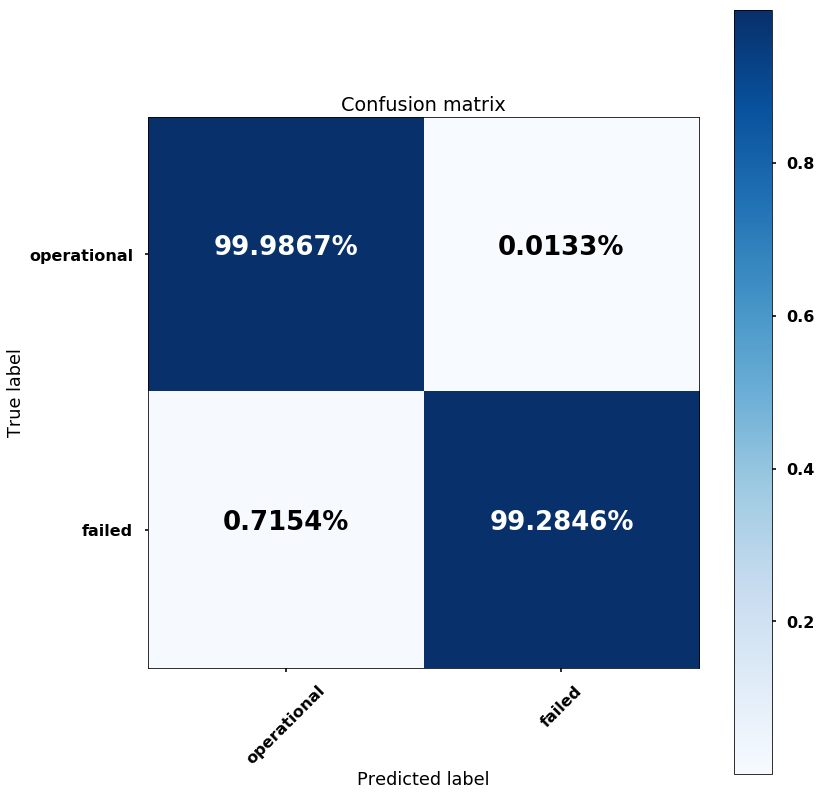
\includegraphics[width=2.5in]{confusion-full-feature}
	\caption{Normalized average confusion matrix of the validation sets of 3-fold cross validation using the full feature set.}
    \label{fig:full-features-confusion-matrix}
\end{subfigure}%
~
\begin{subfigure}[!t]{0.48\textwidth}
	\centering
	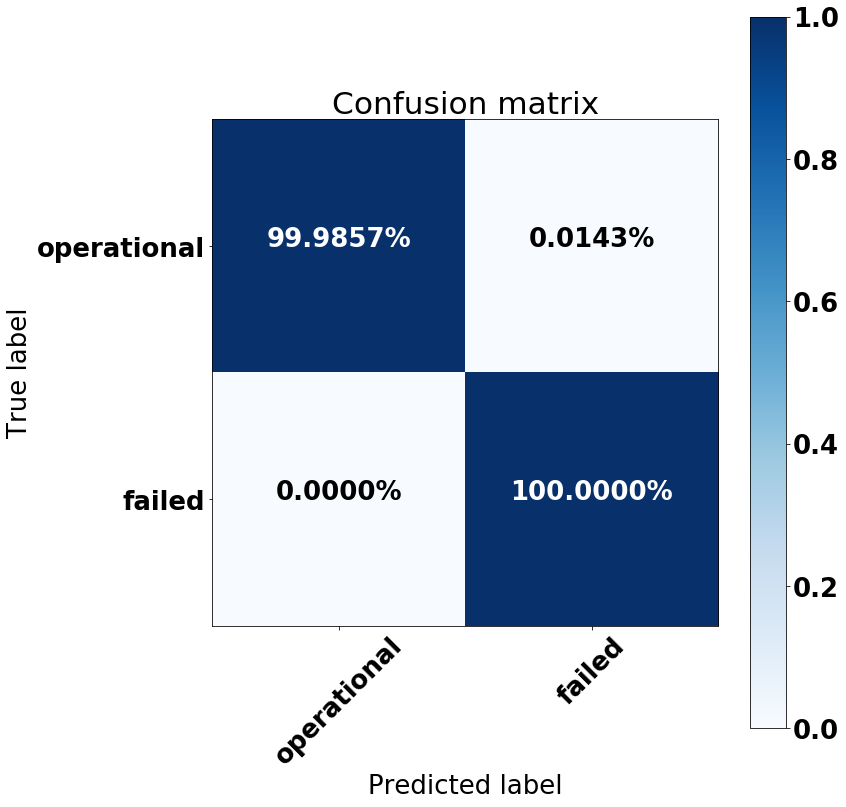
\includegraphics[width=2.5in]{confusion-matrix-1-day-reduced-features}
\caption{Normalized average confusion matrix of the validation sets of 3-fold cross validation using the reduced feature set.}
\label{fig:reduced-features-confusion-matrix}
\end{subfigure}
\caption{Normalized average confusion matrices from the model trained on the full feature set (left) and the reduced feature set (right).}
\end{figure}

The initial formulation of the logistic regression was promising, however, the confusion matrix still had weight on the off-diagonal, predicting machine failures when the machine was still functional or not catching machine failures when they did occur. There was a higher percentage within the confusion matrix for false negatives\textemdash that is, when the logistic regression did not accurately predict failures when they occurred, and the team considered this quality something to be avoided.

\begin{figure}[!ht]
\centering
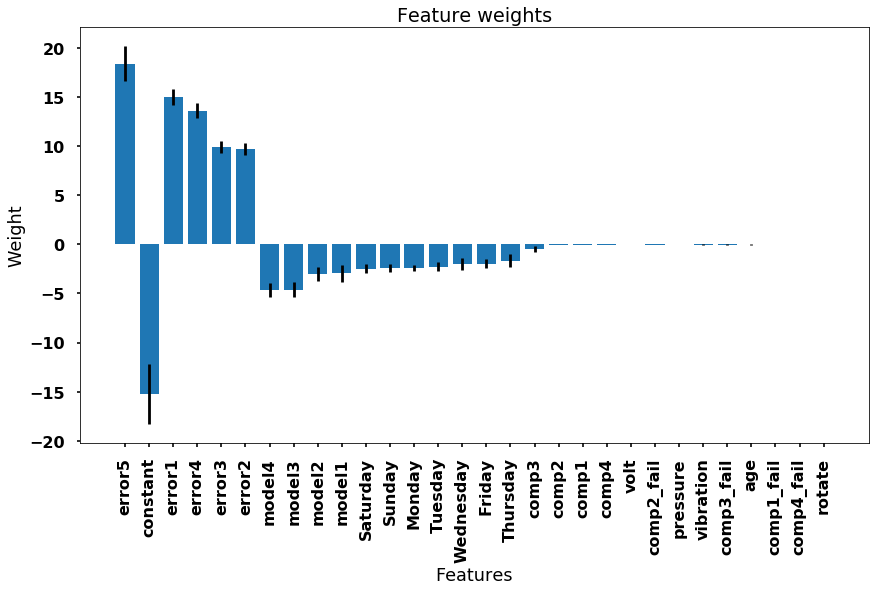
\includegraphics[width=5.5in]{full-feature-weights}
\caption{Average values of the feature weights over 3-fold cross validation ordered by magnitude. The 'constant' feature corresponds to $\alpha$ in \eqref{eqn:logisitic-regression-model} while the rest correspond to elements of $\beta$.}
\label{fig:full-feature-weights}
\end{figure}

Additionally, an examination of the weights used in this logistic regression indicated that there was a large proportion of weights that simply were not significant to the model (see \ref{fig:full-feature-weights}). These included attribute categories like the day of the week, which component was replaced during maintenance, whether the component replace was due to failure, and the telemetry data. This indicated that these variables could be easily removed from the analysis with little consequence.

%This should be after figure 2
It is evident that fewer features affect machine failure than initially understood. The goal is to reduce the frequency of false-negatives by adjusting the size of the $\beta$ vector to represent fewer, but more important, features. Figure \ref{fig:reduced-features-confusion-matrix} shows the confusion matrix of the logistic regression trained on the smaller feature set. By reducing the feature set to included only the most important features, the accuracy of the logistic regression on the held-out data increased. In particular, it reduced the rate of false negatives where the machine was predicted to be operational but in fact has failed.

\section{Discussion}

While logistic regression was utilized in this analysis, there are other machine learning techniques that could be applied. For instance, Support Vector Machine classification (SVM) would have a degree of applicability. This is because SVM is easily applied to highly dimensional spaces and our dataset had 30 attributes per observation. \cite{Cortes1995}

In terms of improvement on the logistic regression, the largest potential is with false positives. That is, while demonstrating (within the test set) 100\% accuracy when it came to predicting failures, the logistic regression predicted failures in machines that were still operational. Thankfully, this is most likely where the margin of safety should be. That is, a machine failing before being caught is most likely more detrimental than a machine being inspected in a controlled environment. Nevertheless, this still is the area where our model is most in need of improvement.

One issue to explore is how sensitive logistic regression is to the time alloted before the point of failure. Currently, a 24 hour period is applied, it is interesting to attempt the logistic regression for both a shorter and longer periods. Therefore, further analysis could investigate whether or not larger periods of time would have comparable (or perhaps even improved) accuracy. Additionally, this additional analysis could incorporate a breadth of data over time.

The current logistic regression does not distinguish between components when a failure is predicted, just machine failure. Thus, further analysis might look into predicting which components will likely fail. Pinpointing component failure may further decrease maintenance costs, as the maintenance team would no longer need to have repairing capabilities for all of the components, just specific failure-prone components.


\section{Acknowledgments}
Our deepest gratitude goes to the Auton Lab at Carnegie Mellon University for providing the data set, and organizing the HackAuton. Additional thanks to the sponsors for providing the funding and datasets to make this HackAuton possible.


\bibliographystyle{plainnat}
\bibliography{sources}

\end{document}

\section{Submission of papers to NIPS 2017}

NIPS requires electronic submissions.  The electronic submission site
is
\begin{center}
  \url{https://cmt.research.microsoft.com/NIPS2017/}
\end{center}

Please read carefully the instructions below and follow them
faithfully.

\subsection{Style}

Papers to be submitted to NIPS 2017 must be prepared according to the
instructions presented here. Papers may only be up to eight pages
long, including figures. This does not include acknowledgments and 
cited references which are allowed on subsequent pages.
Papers that exceed these limits will not be reviewed, or in any
other way considered for presentation at the conference.

The margins in 2017 are the same as since 2007, which allow for
$\sim$$15\%$ more words in the paper compared to earlier years.

Authors are required to use the NIPS \LaTeX{} style files obtainable
at the NIPS website as indicated below. Please make sure you use the
current files and not previous versions. Tweaking the style files may
be grounds for rejection.

\subsection{Retrieval of style files}

The style files for NIPS and other conference information are
available on the World Wide Web at
\begin{center}
  \url{http://www.nips.cc/}
\end{center}
The file \verb+nips_2017.pdf+ contains these instructions and
illustrates the various formatting requirements your NIPS paper must
satisfy.

The only supported style file for NIPS 2017 is \verb+nips_2017.sty+,
rewritten for \LaTeXe{}.  \textbf{Previous style files for \LaTeX{}
  2.09, Microsoft Word, and RTF are no longer supported!}

The new \LaTeX{} style file contains two optional arguments:
\verb+final+, which creates a camera-ready copy, and \verb+nonatbib+,
which will not load the \verb+natbib+ package for you in case of
package clash.

At submission time, please omit the \verb+final+ option. This will
anonymize your submission and add line numbers to aid review.  Please
do \emph{not} refer to these line numbers in your paper as they will
be removed during generation of camera-ready copies.

The file \verb+nips_2017.tex+ may be used as a ``shell'' for writing
your paper. All you have to do is replace the author, title, abstract,
and text of the paper with your own.

The formatting instructions contained in these style files are
summarized in Sections \ref{gen_inst}, \ref{headings}, and
\ref{others} below.

\section{General formatting instructions}
\label{gen_inst}

The text must be confined within a rectangle 5.5~inches (33~picas)
wide and 9~inches (54~picas) long. The left margin is 1.5~inch
(9~picas).  Use 10~point type with a vertical spacing (leading) of
11~points.  Times New Roman is the preferred typeface throughout, and
will be selected for you by default.  Paragraphs are separated by
\nicefrac{1}{2}~line space (5.5 points), with no indentation.

The paper title should be 17~point, initial caps/lower case, bold,
centered between two horizontal rules. The top rule should be 4~points
thick and the bottom rule should be 1~point thick. Allow
\nicefrac{1}{4}~inch space above and below the title to rules. All
pages should start at 1~inch (6~picas) from the top of the page.

For the final version, authors' names are set in boldface, and each
name is centered above the corresponding address. The lead author's
name is to be listed first (left-most), and the co-authors' names (if
different address) are set to follow. If there is only one co-author,
list both author and co-author side by side.

Please pay special attention to the instructions in Section \ref{others}
regarding figures, tables, acknowledgments, and references.

\section{Headings: first level}
\label{headings}

All headings should be lower case (except for first word and proper
nouns), flush left, and bold.

First-level headings should be in 12-point type.

\subsection{Headings: second level}

Second-level headings should be in 10-point type.

\subsubsection{Headings: third level}

Third-level headings should be in 10-point type.

\paragraph{Paragraphs}

There is also a \verb+\paragraph+ command available, which sets the
heading in bold, flush left, and inline with the text, with the
heading followed by 1\,em of space.

\section{Citations, figures, tables, references}
\label{others}

These instructions apply to everyone.

\subsection{Citations within the text}

The \verb+natbib+ package will be loaded for you by default.
Citations may be author/year or numeric, as long as you maintain
internal consistency.  As to the format of the references themselves,
any style is acceptable as long as it is used consistently.

The documentation for \verb+natbib+ may be found at
\begin{center}
  \url{http://mirrors.ctan.org/macros/latex/contrib/natbib/natnotes.pdf}
\end{center}
Of note is the command \verb+\citet+, which produces citations
appropriate for use in inline text.  For example,
\begin{verbatim}
   \citet{hasselmo} investigated\dots
\end{verbatim}
produces
\begin{quote}
  Hasselmo, et al.\ (1995) investigated\dots
\end{quote}

If you wish to load the \verb+natbib+ package with options, you may
add the following before loading the \verb+nips_2017+ package:
\begin{verbatim}
   \PassOptionsToPackage{options}{natbib}
\end{verbatim}

If \verb+natbib+ clashes with another package you load, you can add
the optional argument \verb+nonatbib+ when loading the style file:
\begin{verbatim}
   \usepackage[nonatbib]{nips_2017}
\end{verbatim}

As submission is double blind, refer to your own published work in the
third person. That is, use ``In the previous work of Jones et
al.\ [4],'' not ``In our previous work [4].'' If you cite your other
papers that are not widely available (e.g., a journal paper under
review), use anonymous author names in the citation, e.g., an author
of the form ``A.\ Anonymous.''

\subsection{Footnotes}

Footnotes should be used sparingly.  If you do require a footnote,
indicate footnotes with a number\footnote{Sample of the first
  footnote.} in the text. Place the footnotes at the bottom of the
page on which they appear.  Precede the footnote with a horizontal
rule of 2~inches (12~picas).

Note that footnotes are properly typeset \emph{after} punctuation
marks.\footnote{As in this example.}

\subsection{Figures}

All artwork must be neat, clean, and legible. Lines should be dark
enough for purposes of reproduction. The figure number and caption
always appear after the figure. Place one line space before the figure
caption and one line space after the figure. The figure caption should
be lower case (except for first word and proper nouns); figures are
numbered consecutively.

You may use color figures.  However, it is best for the figure
captions and the paper body to be legible if the paper is printed in
either black/white or in color.
\begin{figure}[h]
  \centering
  \fbox{\rule[-.5cm]{0cm}{4cm} \rule[-.5cm]{4cm}{0cm}}
  \caption{Sample figure caption.}
\end{figure}

\subsection{Tables}

All tables must be centered, neat, clean and legible.  The table
number and title always appear before the table.  See
Table~\ref{sample-table}.

Place one line space before the table title, one line space after the
table title, and one line space after the table. The table title must
be lower case (except for first word and proper nouns); tables are
numbered consecutively.

Note that publication-quality tables \emph{do not contain vertical
  rules.} We strongly suggest the use of the \verb+booktabs+ package,
which allows for typesetting high-quality, professional tables:
\begin{center}
  \url{https://www.ctan.org/pkg/booktabs}
\end{center}
This package was used to typeset Table~\ref{sample-table}.

\begin{table}[t]
  \caption{Sample table title}
  \label{sample-table}
  \centering
  \begin{tabular}{lll}
    \toprule
    \multicolumn{2}{c}{Part}                   \\
    \cmidrule{1-2}
    Name     & Description     & Size ($\mu$m) \\
    \midrule
    Dendrite & Input terminal  & $\sim$100     \\
    Axon     & Output terminal & $\sim$10      \\
    Soma     & Cell body       & up to $10^6$  \\
    \bottomrule
  \end{tabular}
\end{table}

\section{Final instructions}

Do not change any aspects of the formatting parameters in the style
files.  In particular, do not modify the width or length of the
rectangle the text should fit into, and do not change font sizes
(except perhaps in the \textbf{References} section; see below). Please
note that pages should be numbered.

\section{Preparing PDF files}

Please prepare submission files with paper size ``US Letter,'' and
not, for example, ``A4.''

Fonts were the main cause of problems in the past years. Your PDF file
must only contain Type 1 or Embedded TrueType fonts. Here are a few
instructions to achieve this.

\begin{itemize}

\item You should directly generate PDF files using \verb+pdflatex+.

\item You can check which fonts a PDF files uses.  In Acrobat Reader,
  select the menu Files$>$Document Properties$>$Fonts and select Show
  All Fonts. You can also use the program \verb+pdffonts+ which comes
  with \verb+xpdf+ and is available out-of-the-box on most Linux
  machines.

\item The IEEE has recommendations for generating PDF files whose
  fonts are also acceptable for NIPS. Please see
  \url{http://www.emfield.org/icuwb2010/downloads/IEEE-PDF-SpecV32.pdf}

\item \verb+xfig+ "patterned" shapes are implemented with bitmap
  fonts.  Use "solid" shapes instead.

\item The \verb+\bbold+ package almost always uses bitmap fonts.  You
  should use the equivalent AMS Fonts:
\begin{verbatim}
   \usepackage{amsfonts}
\end{verbatim}
followed by, e.g., \verb+\mathbb{R}+, \verb+\mathbb{N}+, or
\verb+\mathbb{C}+ for $\mathbb{R}$, $\mathbb{N}$ or $\mathbb{C}$.  You
can also use the following workaround for reals, natural and complex:
\begin{verbatim}
   \newcommand{\RR}{I\!\!R} %real numbers
   \newcommand{\Nat}{I\!\!N} %natural numbers
   \newcommand{\CC}{I\!\!\!\!C} %complex numbers
\end{verbatim}
Note that \verb+amsfonts+ is automatically loaded by the
\verb+amssymb+ package.

\end{itemize}

If your file contains type 3 fonts or non embedded TrueType fonts, we
will ask you to fix it.

\subsection{Margins in \LaTeX{}}

Most of the margin problems come from figures positioned by hand using
\verb+\special+ or other commands. We suggest using the command
\verb+\includegraphics+ from the \verb+graphicx+ package. Always
specify the figure width as a multiple of the line width as in the
example below:
\begin{verbatim}
   \usepackage[pdftex]{graphicx} ...
   \includegraphics[width=0.8\linewidth]{myfile.pdf}
\end{verbatim}
See Section 4.4 in the graphics bundle documentation
(\url{http://mirrors.ctan.org/macros/latex/required/graphics/grfguide.pdf})

A number of width problems arise when \LaTeX{} cannot properly
hyphenate a line. Please give LaTeX hyphenation hints using the
\verb+\-+ command when necessary.

\subsubsection*{Acknowledgments}

Use unnumbered third level headings for the acknowledgments. All
acknowledgments go at the end of the paper. Do not include
acknowledgments in the anonymized submission, only in the final paper.

\section*{References}

References follow the acknowledgments. Use unnumbered first-level
heading for the references. Any choice of citation style is acceptable
as long as you are consistent. It is permissible to reduce the font
size to \verb+small+ (9 point) when listing the references. {\bf
  Remember that you can go over 8 pages as long as the subsequent ones contain
  \emph{only} cited references.}
\medskip

\small

[1] Alexander, J.A.\ \& Mozer, M.C.\ (1995) Template-based algorithms
for connectionist rule extraction. In G.\ Tesauro, D.S.\ Touretzky and
T.K.\ Leen (eds.), {\it Advances in Neural Information Processing
  Systems 7}, pp.\ 609--616. Cambridge, MA: MIT Press.

[2] Bower, J.M.\ \& Beeman, D.\ (1995) {\it The Book of GENESIS:
  Exploring Realistic Neural Models with the GEneral NEural SImulation
  System.}  New York: TELOS/Springer--Verlag.

[3] Hasselmo, M.E., Schnell, E.\ \& Barkai, E.\ (1995) Dynamics of
learning and recall at excitatory recurrent synapses and cholinergic
modulation in rat hippocampal region CA3. {\it Journal of
  Neuroscience} {\bf 15}(7):5249-5262.

\end{document}